%=================================================================
% Security companion paper (Paper F of the bundle): threat model, tamper
% detectability, operating points, and structural limits for the sensor-side
% G-code integrity monitor whose recoverability foundation is the companion
% decoder paper. Assembled 2026-08-13 from the certified v4 threat-model
% sections + v2 supplement extended operating-point/deployment sections.
% Compile from this directory: pdflatex; bibtex security_companion; pdflatex x2.
%=================================================================
\documentclass[sensors,article,submit,moreauthors,pdftex]{Definitions/mdpi}

%=================================================================
% MDPI frontmatter
\firstpage{1}
\makeatletter
\setcounter{page}{\@firstpage}
\makeatother
\pubvolume{1}
\issuenum{1}
\articlenumber{0}
\pubyear{2026}
\copyrightyear{2026}
\history{}

%=================================================================
% Packages
\usepackage{siunitx}
\usepackage{multirow}
\usepackage{booktabs}
\usepackage{enumitem}
\usepackage{subcaption}
\usepackage{graphicx}
\usepackage{float}
\setlength{\intextsep}{3pt plus 1pt minus 1pt}
\setlength{\textfloatsep}{6pt plus 1pt minus 2pt}
\setlength{\abovecaptionskip}{4pt}
\AtBeginDocument{\setlength{\bibsep}{0pt}\renewcommand{\bibfont}{\footnotesize}}
\graphicspath{{../figures/}}

% Custom commands
\newcommand{\modelname}{G-Code Decoder}
\newcommand{\encname}{MM-DTAE-LSTM}
\newcommand{\ie}{\textit{i.e.}}
\newcommand{\eg}{\textit{e.g.}}
\newcommand{\etal}{\textit{et al.}}

% MDPI back-matter macros not present in the local (older) mdpi.cls.
\providecommand{\institutionalreview}[1]{\medskip\noindent\textbf{Institutional Review Board Statement:} #1\par}
\providecommand{\informedconsent}[1]{\medskip\noindent\textbf{Informed Consent Statement:} #1\par}
\providecommand{\dataavailability}[1]{\medskip\noindent\textbf{Data Availability Statement:} #1\par}

%=================================================================
% Title
\Title{Sensor-Side Tamper Detection for CNC Machining: Threat Model, Illustrative Operating Points, and Structural Limits of a G-Code Recoverability Monitor}

\newcommand{\orcidauthorA}{0009-0009-0292-9706}

\Author{Stephen S. Eacuello $^{1,}$*\orcidA{}, Romesh S. Prasad $^{1}$ and Manbir S. Sodhi $^{1}$}

\AuthorNames{Stephen S. Eacuello, Romesh S. Prasad and Manbir S. Sodhi}

\address{%
$^{1}$ \quad Department of Industrial and Systems Engineering, University of Rhode Island, Kingston, RI 02881, USA}

\corres{Correspondence: seacuello@uri.edu}

\abstract{
A controller-resident adversary can alter the executed G-code without altering the loaded file, so file signing and attestation leave execution unverified. We analyze whether an out-of-band sensor-side monitor can verify the executed instruction stream, using companion per-field G-code recoverability measurements on a desktop CNC mill's 4~Hz multi-modal stack. We formalize the threat model (five attack classes, MITRE ATT\&CK for ICS-mapped) and report per-attack-class detectability with synthetic tamper-injection operating points on 5-fold predictions. Command-swap detection reaches balanced accuracy $0.81$ ($0.86$ with metadata); sign-flip and feed-rate detection are largely prior-driven, collapsing under the open-vocabulary regime. At the measured honest-side autocorrelation ($\rho = 0.42$), a $K{=}10$ majority aggregation with metadata reaches FPR $0.098$ at TPR $0.97$ for analyst triage; per-window alerting yields hundreds of alerts per machine-shift, several times a tier-1 analyst budget. Detection is prior-dominated: the sensor-conditioned lift is $\sim$$8$~pp TPR over a sensor-independent corpus-modal control. On unseen operation classes the command-swap detector collapses to FPR $0.52$, and an adversary who corrupts only fine-grained coordinates or feed rate is invisible by construction. The operating points are illustrative, not a validated detector; the supported posture is forensic-support post-hoc audit in a single-platform, closed-world scope.
}

\keyword{manufacturing cybersecurity; tamper detection; CNC machining; threat model; side-channel; forensic audit; industrial control systems; G-code}

\begin{document}

% =====================================================================
\section{Introduction}
\label{sec:introduction}

A Computer Numerical Control (CNC) controller executes G-code programs that determine part geometry, feed, and spindle behavior. A controller-resident adversary with write access to program memory can substitute instructions at runtime while the loaded file, and therefore its cryptographic hash, remains unchanged~\cite{sturm2014cyber,yampolskiy2018security,kimmell2025cnc}. File signing verifies the program at rest and controller attestation verifies the boot chain, but neither extends to what the machine physically executed. The FMNet 2024 research-needs report~\cite{nist2024fmnet} identifies this machining-specific instruction-stream-integrity gap.

An out-of-band monitor that reconstructs the executed instruction stream from external sensors would provide an integrity baseline that controller-resident malware cannot subvert, subject to the sensor path itself being trustworthy. A companion study~\cite{decoder_paper} measured the precondition for such a monitor: which fields of an executing G-code block are recoverable from a 4~Hz seven-modality sensor stream on a desktop CNC mill. Its central result is a factorization: categorical structure (command identity, axis presence, motion sign) is recoverable within a closed-vocabulary, in-distribution envelope, while numeric coordinate values and feed rate are not, with generative whole-line reconstruction at floor. The present paper develops what that factorization implies for security: which attacks such a monitor can and cannot see, at what operating points, at what alert cost, and against which adversaries.

The analysis yields a deliberately bounded conclusion, stated up front. The tamper operating points reported here are \emph{illustrative}, derived from synthetic relabelling of honest predictions rather than physically executed attacks, and the detection signal is \emph{prior-dominated}: most of the row-level detectability is a property of the closed-vocabulary command prior rather than per-instruction sensor recovery. Window-level alerting exceeds a realistic Security Operations Center (SOC) per-analyst alert budget several-fold per machine, detection collapses outside the trained operation-class envelope, and an adversary who corrupts only the fields the sensor stack cannot recover bypasses the monitor by construction. The supported deployment posture is forensic-support post-hoc audit of contested runs, not real-time intrusion detection.

\paragraph{Contributions.}
\begin{enumerate}[label=\textbf{(\arabic*)}, leftmargin=*]
\item A \textbf{threat model} for sensor-side G-code execution verification: trusted and untrusted elements, five attack classes mapped to the MITRE ATT\&CK for ICS taxonomy~\cite{mitre_attack_ics}, and the monitor's position in the NIST CSF~2.0 Detect function~\cite{nistcsf2} (Section~\ref{sec:threat-model}).
\item A \textbf{per-attack-class detectability map} derived from the companion study's measured per-field recoverability~\cite{decoder_paper}, including the boundary cases (Section~\ref{sec:detectability}).
\item \textbf{Illustrative tamper-injection operating points} on 5-fold autoregressive predictions for command-swap, sign-flip, and feed-rate attacks, under both the in-distribution and open-vocabulary leave-one-class-out regimes (the positional-metadata effect and its trust-boundary tension are measured in-distribution; Section~\ref{sec:operating-points}).
\item An \textbf{alert-budget and aggregation analysis} at the empirically measured alert autocorrelation, a sensor-versus-prior control quantifying how much of the detection is prior structure, and the open-vocabulary collapse (Section~\ref{sec:alert-budget}).
\item An \textbf{adaptive-adversary analysis} showing the monitor's blind spots define a structural bypass, with the sensor-side adversary scope and operational mitigations (Section~\ref{sec:adaptive}).
\item A \textbf{deployment posture}: two operating points for forensic-support post-hoc audit and human-in-the-loop triage, and the defense-in-depth position relative to file signing and attestation (Section~\ref{sec:deployment}).
\end{enumerate}

Every quantitative result is conditional on the companion study's single desktop platform, material, and 4~Hz sensor stream~\cite{decoder_paper}; no physical tamper was executed, and no result here upgrades the monitor to a validated detector.

% =====================================================================
\section{Related Work}
\label{sec:related}

Adversarial G-code substitution in PLC and CNC controllers is an established attack surface~\cite{zonouz2014plc,sturm2014cyber,yampolskiy2018security,kimmell2025cnc}. Belikovetsky \etal~\cite{belikovetsky2017drowned} demonstrated an end-to-end additive-manufacturing sabotage attack that survived file-level review, and file-hash signing is the standard countermeasure at the file-at-rest layer~\cite{belikovetsky2017drowned,nist2024fmnet}; controller attestation addresses the boot chain~\cite{zonouz2014plc}. NIST SP~800-82~Rev.~3~\cite{nist2023sp80082} provides the operational-technology framing, with continuous monitoring under the Detect function and supply-chain-risk guidance. Against that framing an out-of-band physics-of-record monitor is a complementary control whose guarantee holds only insofar as the sensor path is trustworthy.

Side-channel analysis of manufacturing equipment established that executed toolpaths leak through physical emissions: acoustic~\cite{alfaruque2016acoustic,song2016my}, kinetic~\cite{chhetri2016kcad}, optical~\cite{chattopadhyay2025video}, and combined acoustic-magnetic~\cite{jamarani2024screg} channels reconstruct additive-manufacturing geometry, typically from kHz--MHz raw signals. Kimmell \etal~\cite{kimmell2025cnc} detect CNC control-injection attacks via energy-anomaly thresholds, a binary detection target; session-level anomaly classifiers~\cite{coelho2024anomaly} similarly flag whole runs. The companion study~\cite{decoder_paper} differs in target granularity, recovering per-row, per-field instruction content from a 4~Hz envelope stream, and the present paper is the security analysis built on that recovery. The defense-in-depth division of labor is analyzed in Section~\ref{sec:deployment}: file signing, attestation, and the sensor-side monitor each cover attack classes the others cannot.

% =====================================================================
\section{Threat Model}
\label{sec:threat-model}

\paragraph{Trusted elements.} The multi-modal sensor stack and its acquisition pipeline are trusted: sensors are physically secured, the telemetry path is integrity-protected, the recorded sensor stream faithfully represents the physical machine state, and the decoder model and verification host are not co-located with the controller. These are operational requirements on a deployment, not features of the present prototype (the laboratory pipeline uses unauthenticated USB sensor links). Trusting the sensor path is realistic when sensors and analysis live outside the controller's trust boundary, but it is a non-trivial operational assumption (Section~\ref{sec:adaptive}). A controller-resident adversary with bus access to shared sensor infrastructure is out of scope, as are sensor-side wire-tap, EMI injection, packet replay, and calibration-spoofing attacks. We additionally assume that the operator who initiates each run is authenticated to the verification host and that the program loaded on the controller is the same artifact whose hash was audited. An insider-threat operator who loads an unaudited program after attestation is a residual adversary the present scope does not address.

\paragraph{Untrusted elements.} The CNC controller, its firmware, and any G-code dispatch path between controller and machine are untrusted. The adversary may have read/write access to the controller's program memory, may inject substituted G-code, may modify cutting parameters mid-execution, or may replay an earlier benign program while a different program is intended.

\paragraph{Attack classes considered.} We consider five attack classes: (i)~\emph{block substitution} (e.g., \texttt{G1 X1.5} becomes \texttt{G1 X2.5}; substituted blocks may differ in command identity, axis, sign, or numeric value); (ii)~\emph{parameter tampering}, in which the program is structurally preserved but cutting parameters (feed, spindle speed, depth of cut) are altered; (iii)~\emph{replay} of a previously-executed valid program while a different program was commanded; (iv)~\emph{block skip or duplicate} of executed blocks while the controller log reports nominal execution; and (v)~\emph{upstream CAM / post-processor compromise}, in which the toolpath is corrupted before the operator-signed G-code file is produced. Class~(v) is enumerated for completeness but is out of scope for the present monitor, which agrees with an already-corrupted controller stream (Section~\ref{sec:adaptive}). Detectability for the substitution classes and the feed-rate component of parameter tampering is reported in Table~\ref{tab:tamper_auc} (spindle-speed recovery is not evaluable on the companion corpus); classes (iii)--(iv) are assessed qualitatively in Section~\ref{sec:detectability} and class (v) in Section~\ref{sec:adaptive}. In the MITRE ATT\&CK for ICS taxonomy~\cite{mitre_attack_ics} these classes map respectively to T0843 / T0889 (Program Download / Modify Program), T0836 / T0831 (Modify Parameter / Manipulation of Control), T0855 (Unauthorized Command Message, covering replayed command traffic), T0856 (Spoof Reporting Message, covering execution the log misreports), and T0862 (Supply Chain Compromise). The monitor occupies the \emph{Detect} function of NIST CSF~2.0 (continuous-monitoring category DE.CM)~\cite{nistcsf2}, complementing prevention controls (file signing, attestation) rather than replacing them. \emph{Protect}, \emph{Respond}, and \emph{Recover} remain out of scope.

\paragraph{Adversary model: orthogonal defenses.} The sensor-side monitor is intended to run in parallel with the cheaper orthogonal defenses (file-hash / cryptographic signature on the G-code file; trusted-computing-base attestation on the controller), not in place of them. Each defense covers attack classes the others cannot. The monitor's residual value is the attack subset that survives a signed-G-code audit and defeats controller attestation that does not extend to runtime memory: runtime command/axis/sign substitution. Within that subset, the monitor is further bounded by the closed-vocabulary in-distribution regime under which the underlying decoder is trained~\cite{decoder_paper} and by the per-field recoverability summarized next.

% =====================================================================
\section{The Recoverability Foundation}
\label{sec:foundation}

The companion study~\cite{decoder_paper} trains a six-head Transformer decoder with grammar-constrained inference on the frozen latent of a prior multi-modal denoising encoder~\cite{encoder_paper} (nine-class operation accuracy $96.3\%$), using a hybrid grammar tokenization~\cite{grammar_paper}, and evaluates per-field G-code recovery under five-fold file-level cross-validation on a 120-file corpus from one desktop CNC mill (air-cut and UHMW-PE active-cut runs; seven sensor modalities, 98 channels, 4~Hz envelope-extracted stream). Four of its measured results carry the security analysis.

First, \emph{categorical structure is recoverable in-distribution under reference-conditioned (teacher-forced) evaluation}: command accuracy is $0.8875 \pm 0.0558$, parameter-type $0.9931 \pm 0.0036$, and pooled motion-sign $0.9888 \pm 0.0063$; measured free-running categorical accuracy collapses (command $0.483 \pm 0.049$)~\cite{decoder_paper}, so the categorical signal requires conditioning on a reference stream, which in the audit posture the controller log provides. The pooled sign figure is prior-dominated: only the Z axis carries non-trivial sign information ($H_{Z}^{\text{sign}}\!=\!1.04$~bits vs.\ $H_{Y}^{\text{sign}}\!=\!0.08$, $H_{X}^{\text{sign}}\!=\!0.38$)~\cite{paperB_entropy}.

Second, \emph{the categorical signal itself is largely class-prior structure}: against a history-free operation-class modal predictor ($0.572$), the decoder reaches $0.795 \pm 0.121$ at command-token positions, a $+22$~pp within-class increment ($\approx\!+13$~pp against a history-matched Markov null, $0.662$) that is an upper bound on sensor-driven recovery, is at or below the class prior on one covariate-shift outlier fold, and is unchanged under a test-derived class-modal null ($0.576$)~\cite{decoder_paper}.

Third, \emph{numeric precision and feed rate are not recoverable}: per-digit accuracy bottoms at $0.42$ at the thousandths place --- the finest digit the companion study's tokenizer retains (the CAM source carries a fourth decimal the $0.001$ grid discards) --- a floor the companion limit paper~\cite{paperB_entropy} accounts for information-theoretically; feed-rate recovery is evaluable only in the full-window regime at thin support. Generative whole-sequence reconstruction is at floor (autoregressive exact-match $0.026$).

Fourth, \emph{recovery does not survive novel operation classes}: under leave-one-class-out (LOCO) evaluation, command accuracy collapses from $0.888$ to $0.213 \pm 0.191$~\cite{decoder_paper}. Every closed-vocabulary operating point below must be read against this open-vocabulary floor.

% =====================================================================
\section{Detectability by Attack Class}
\label{sec:detectability}

The per-field recoverability maps onto the attack classes as follows. \emph{Command-identity} (G0$\to$G1) and \emph{axis-identity} (X$\to$Y) substitutions are \emph{detectable} (reference-conditioned accuracies $0.8875 \pm 0.0558$ command, $0.9931 \pm 0.0036$ parameter-type; the detector's own AR-mode operating points are in Table~\ref{tab:tamper_auc}). \emph{Motion-sign} substitution is \emph{partially detectable}: only Z-sign carries non-trivial sensor signal, and Y/X sign ``detection'' is prior mismatch ($H_{Y}^{\text{sign}}\!=\!0.08$, $H_{X}^{\text{sign}}\!=\!0.38$ vs.\ $H_{Z}^{\text{sign}}\!=\!1.04$~bits). \emph{Numeric-value} tampering is \emph{not detectable at fine precision} by an information-theoretic bound (thousandths source entropy $\approx 3.3$~bits, slot-4 accuracy $0.42$)~\cite{paperB_entropy}. \emph{Feed-rate} recovery is evaluable only at thin support and \emph{spindle-speed} recovery is not evaluable on the companion corpus; the $\pm 10\times$ feed-edit rows of Table~\ref{tab:tamper_auc} probe gross synthetic deviations at a $>\!50\%$ threshold, not corpus-supported feed-rate recovery. \emph{Replay} is detectable indirectly: a replayed program that differs from the commanded one would surface as sustained command/axis disagreement against the commanded log over the run, an argument we state as interpretation and do not benchmark. \emph{Skip/duplicate} at per-row granularity is not directly addressed.

Three boundary cases qualify this map. Coarse numeric tampering on the integer or tenths place may be detectable in-distribution when the perturbed value falls outside the per-operation-class value range observed in training. Novel command tokens are either masked by the finite-state grammar layer or fall through to the modal class, so the per-instruction sensor evidence is not consulted against an unrecognized token. Skip/duplicate detection via temporal alignment between sensor windows and the controller log is operationally feasible but not benchmarked here.

% =====================================================================
\section{Illustrative Tamper Operating Points}
\label{sec:operating-points}

\noindent\textbf{The operating points in this section are illustrative, not a validated detector.} No physical tamper was performed. The ``tamper'' is a synthetic relabelling of the honest predictions, and the reported false-alarm rate is mechanically the recoverability complement (one minus per-field recoverability) on the same population, not an independent honest-run-pair measurement. A genuine independent false-alarm estimate (scoring one honest run's predictions against a \emph{different} honest run's controller log, same operation class) requires per-file decoder inference not persisted in the released artifacts and is left to future artifact releases; the recoverability-complement rate is the disclosed proxy here. The detection signal is also \emph{prior-dominated} (Section~\ref{sec:alert-budget}). The numbers make the per-field characterization concrete in attack terms; they do not constitute a deployable detector.

\paragraph{Tamper-injection protocol.} We ran a synthetic tamper-injection audit on the companion study's 5-fold full-window predictions under autoregressive deployment-true decoding with the finite-state grammar layer enabled~\cite{decoder_paper}. For each held-out sample we form the honest pair $(g_{\text{true}}, g_{\text{pred}})$ and mutate $g_{\text{true}}$ by command swap, motion-sign flip on the first signed axis, or feed-rate $\pm 10\times$ edit; a tamper is flagged when the relevant token-class in $g_{\text{pred}}$ differs (thresholds: exact match for command/sign, $>50\%$ relative deviation for F; $n\!=\!483$ command-swap, $549$ sign-flip, $111$ feed-edit pooled). Table~\ref{tab:tamper_auc} reports the balanced accuracy and threshold-matched operating point per attack class (baseline / with-metadata) under both the in-distribution closed-vocabulary and the open-vocabulary LOCO regimes; command-swap is the strongest attack class in both regimes --- moderately discriminable in-distribution --- and every detector degrades under LOCO. The sign-flip and feed-rate detectors carry little sensor signal under autoregressive decoding (sign-flip rides the $99\%$-positive Y prior; feed-rate transients cannot be resolved by the 4-Hz stack) and are non-detectable under LOCO.

\begin{table}[!htbp]
\centering
\caption{Tamper-detection discrimination summary and threshold-matched operating point by attack class, regime, and configuration (``Baseline'' = no positional metadata; ``Metadata'' = window-index/source-file exposed; AR deployment-true decoding with FSM grammar). The released detector is single-threshold (a binary per-window disagreement flag), so every row reports the balanced-accuracy estimator BA$=\!\tfrac{1}{2}(\mathrm{TPR}+(1-\mathrm{FPR}))$; no swept-threshold ROC exists for the binary score. FPR is the recoverability-complement disagreement rate on the unmutated honest pair (Section~\ref{sec:operating-points}). Sources: \texttt{audit/threat\_model\_tamper\_AR\_5fold\_FSM.json} (baseline rows), \texttt{audit/threat\_model\_tamper\_AR\_5fold\_FSM\_shortcuts.json} (metadata rows), \texttt{audit/threat\_model\_tamper\_loco.json} (LOCO rows).}
\label{tab:tamper_auc}
\footnotesize
\setlength{\tabcolsep}{4pt}
\begin{tabular}{l l c c c}
\toprule
\textbf{Attack class} & \textbf{Config.} & \textbf{BA} & \textbf{TPR} & \textbf{FPR} \\
\midrule
\multicolumn{5}{l}{\emph{In-distribution closed-vocabulary regime (5-fold pooled)}} \\
Command-swap (G0$\to$G1)    & Baseline & $0.81$ & $0.921$ & $0.299$ \\
Command-swap                & Metadata  & $0.86$ & $0.948$ & $0.222$ \\
Sign-flip (first signed axis) & Baseline & $0.68$ & $0.703$ & $0.350$ \\
Sign-flip                   & Metadata  & $0.78$ & $0.798$ & $0.244$ \\
Feed-rate $\pm 10\times$    & Baseline & $0.61$ & $0.216$ & $0.0055$ \\
Feed-rate $\pm 10\times$    & Metadata  & $0.76$ & $0.532$ & $0.0146$ \\
\midrule
\multicolumn{5}{l}{\emph{Open-vocabulary leave-one-class-out (LOCO) regime}} \\
Command-swap                & Baseline & $0.66$ & $0.847$ & $0.519$ \\
Sign-flip                   & Baseline & $0.20$ \tiny{(anti-disc.)} & $0.138$ & $0.748$ \\
Feed-rate $\pm 10\times$    & Baseline & $0.50$ \tiny{(degenerate, $n\!=\!45$)} & $0.000$ & $0.000$ \\
\bottomrule
\end{tabular}
\end{table}

The pooled sign-flip TPR/FPR mixes prior-driven detection on Y and X with sensor-driven detection on Z; on Y the $99\%$-positive prior alone explains essentially all of the head's accuracy ($H_{Y}^{\text{sign}}=0.08$~bits), and X is near-deterministic as well. Autoregressive mode collapse strips per-axis-sign and per-feed-rate information, and the pessimistic reading of the sign-flip and feed-rate rows is their alert-budget cost. Figure~\ref{fig:tamper-roc-pair} shows the ROC-space aggregation operating points.

\begin{figure}[!htbp]
\centering
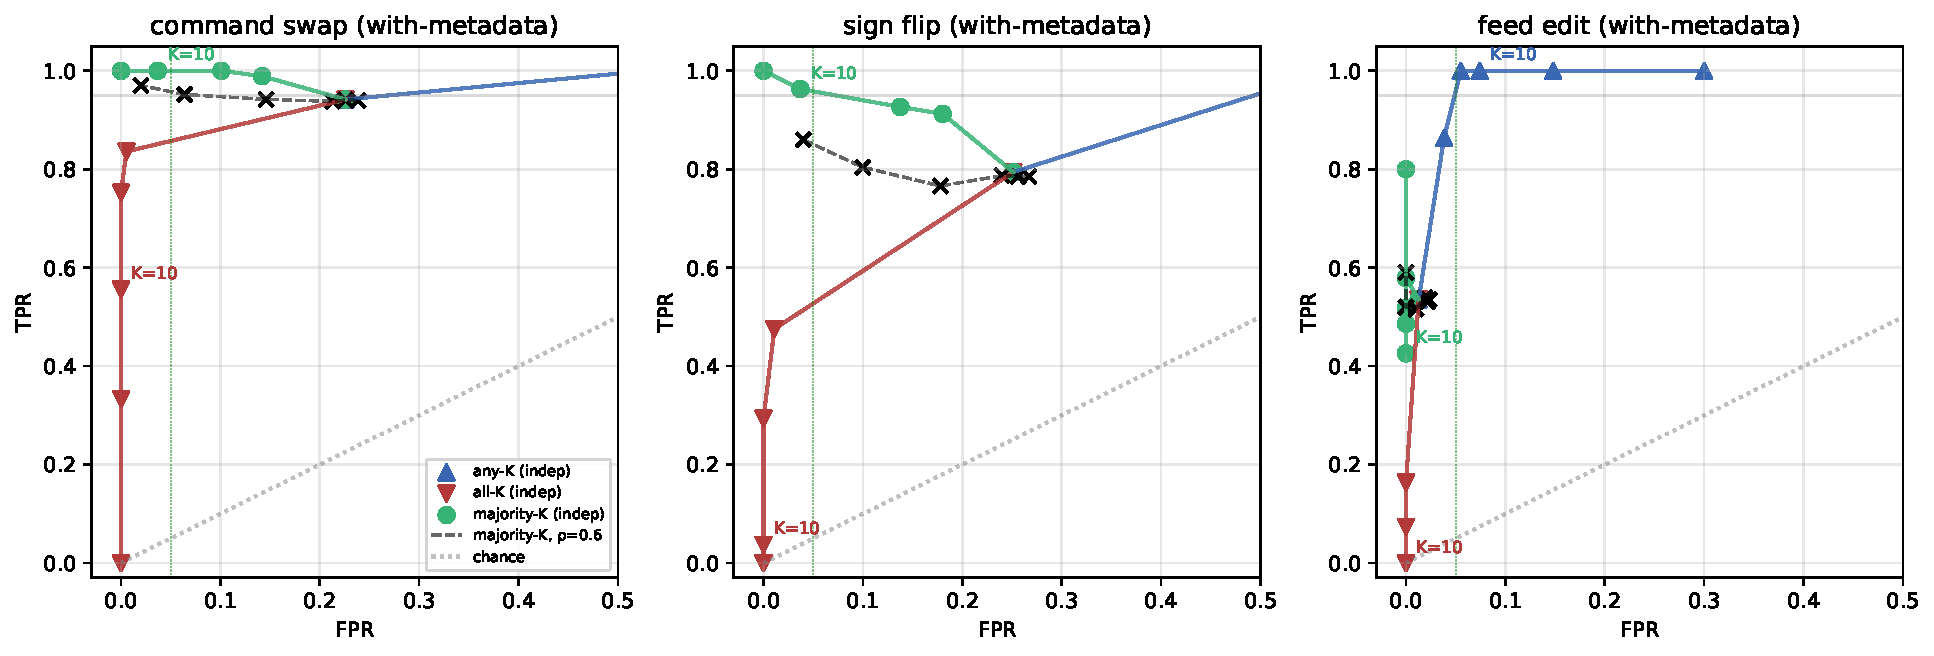
\includegraphics[width=0.6\linewidth]{tamper_roc_scatter.pdf}
\caption{ROC-space aggregation operating points (with-metadata); curves trace $K\!\in\!\{1,3,5,10,20,50\}$; dashed black is a $\rho=0.6$ majority-of-K reference drawn before the measurement (Section~\ref{sec:alert-budget} uses the measured $\rho=0.42$). Security claims are bounded by the open-vocabulary LOCO command-swap point (FPR $0.52$/TPR $0.85$).}
\label{fig:tamper-roc-pair}
\end{figure}

\paragraph{The positional-metadata effect and its trust-boundary tension.} Adding positional metadata strictly improves tamper detection on every attack class (Table~\ref{tab:tamper_auc}; the feed-rate TPR improves $\sim$$2.5\times$). This mirrors the mode-collapse-mitigation finding of the companion study~\cite{decoder_paper}: the per-window anchor that breaks the corpus-modal trajectory also makes predictions discriminative enough to separate tampered from honest logs. The with-metadata configuration is therefore preferable for security use, with one caveat: window-index/source-file metadata is controller-derived while the controller is the untrusted element, a residual trust-boundary tension. Where metadata is unavailable or a sensors-only baseline is needed, the no-metadata configuration is the conservative choice.

% =====================================================================
\section{Alert Budget, Aggregation, and the Prior-Dominance Control}
\label{sec:alert-budget}

\paragraph{False-alarm cost.} The baseline command-swap operating point is TPR $0.92$ at FPR $0.30$ (with-metadata: TPR $0.95$ at FPR $0.22$); the sign-flip operating point is TPR $0.70$/$0.80$ at FPR $0.35$/$0.24$. The detector operates per 64-second window ($\sim$60 G-code rows per window on average~\cite{decoder_paper}). At the corpus window stride of $16$~s, one CNC running an 8-hr shift produces $\sim$$1{,}800$ window decisions; at the with-metadata in-distribution FPR $0.222$ this is $\sim$$400$ alerts/shift/machine (open-vocabulary LOCO FPR $0.519$: $\sim$$930$), several times a working SOC tier-1 alert budget of $\le\!10^{2}$ per analyst per shift, an assumption we adopt consistent with NIST SP~800-61~Rev.~2~\cite{nist2012sp80061} incident-handling capacity planning, and multiplicative in the number of monitored machines. A window-level verification monitor is therefore not viable as the SOC-consumer interface without an aggregation or triage stage. Three candidate mitigations exist, and none yields a window-level operating point that survives the measured-autocorrelation, prior-driven, and open-vocabulary qualifiers established in this section: \emph{(a)}~aggregation over $K$ adjacent window decisions, evaluated next; \emph{(b)}~a fixed-low-false-alarm operating point, which would require a confidence-scored detector the released artifacts do not provide (Section~\ref{sec:deployment}); and \emph{(c)}~temperature-scaled calibration of the command head, which reduces the deployment-relevant cross-fold expected calibration error from $0.050$ to $0.020$ and would supply calibrated confidences to a future scored detector (the released detector is a binary flag; \texttt{audit/calibration\_cross\_fold.json}). The operating points of Table~\ref{tab:tamper_auc} are the threshold-matched first-pass numbers without these enhancements.

\paragraph{Aggregation under the independence idealization.} A Monte-Carlo $K$-window aggregation (any/all/majority-of-K, $K\!\in\!\{1,3,5,10,20,50\}$; \texttt{audit/tamper\_aggregation\_sweep.json}) shows the majority-of-$K$ rule produces an optimistic command-swap point that holds \emph{only} under the (false) window-independence assumption (with-metadata $K\!=\!10$: TPR $1.00$, FPR $\sim\!0.04$); sign-flip benefits weakly and feed-rate not at all (Figure~\ref{fig:agg-curves}). The measured-autocorrelation analysis below replaces this row-independent best case with the deployment-relevant number.

\begin{figure}[!htbp]
\centering
\begin{subfigure}{0.52\linewidth}\centering
  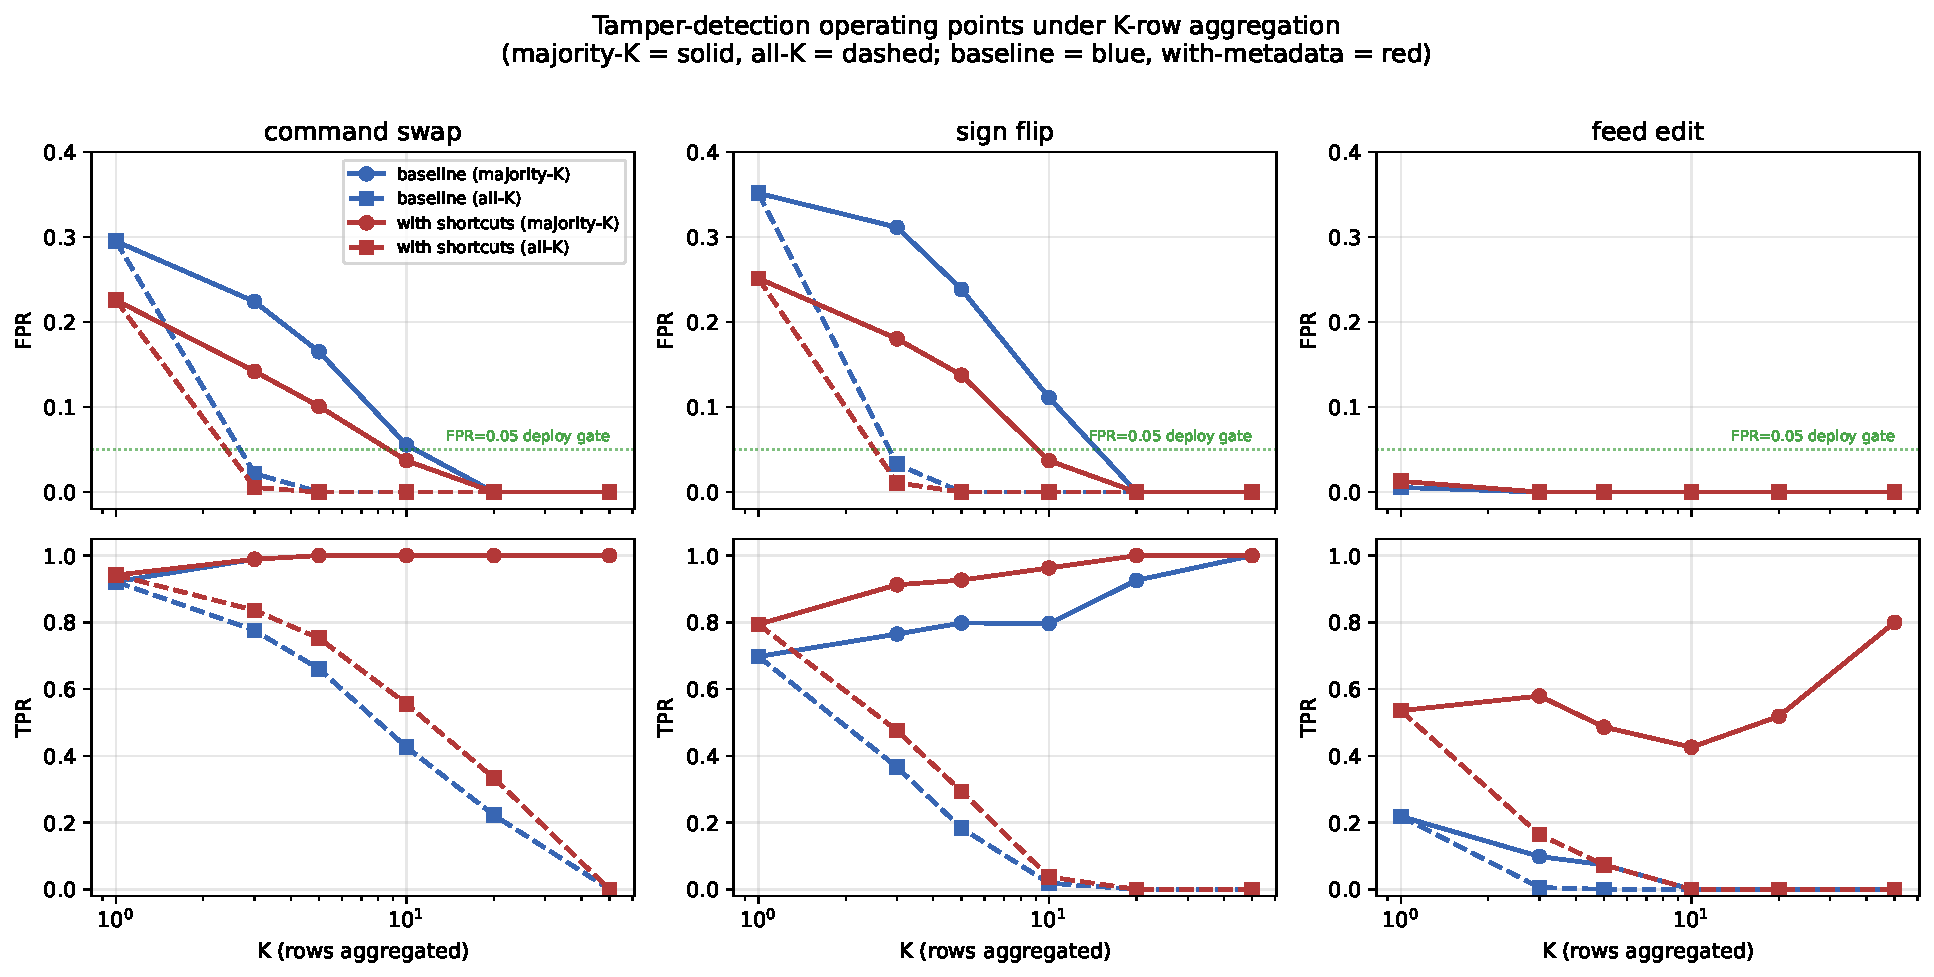
\includegraphics[width=\linewidth]{tamper_aggregation_curves.pdf}
  \caption{$K$-window aggregation curves (any/all/majority-of-$K$) under the independence idealization; the majority-of-$K$ optimism does not survive the measured autocorrelation.}
  \label{fig:agg-curves}
\end{subfigure}\hfill
\begin{subfigure}{0.44\linewidth}\centering
  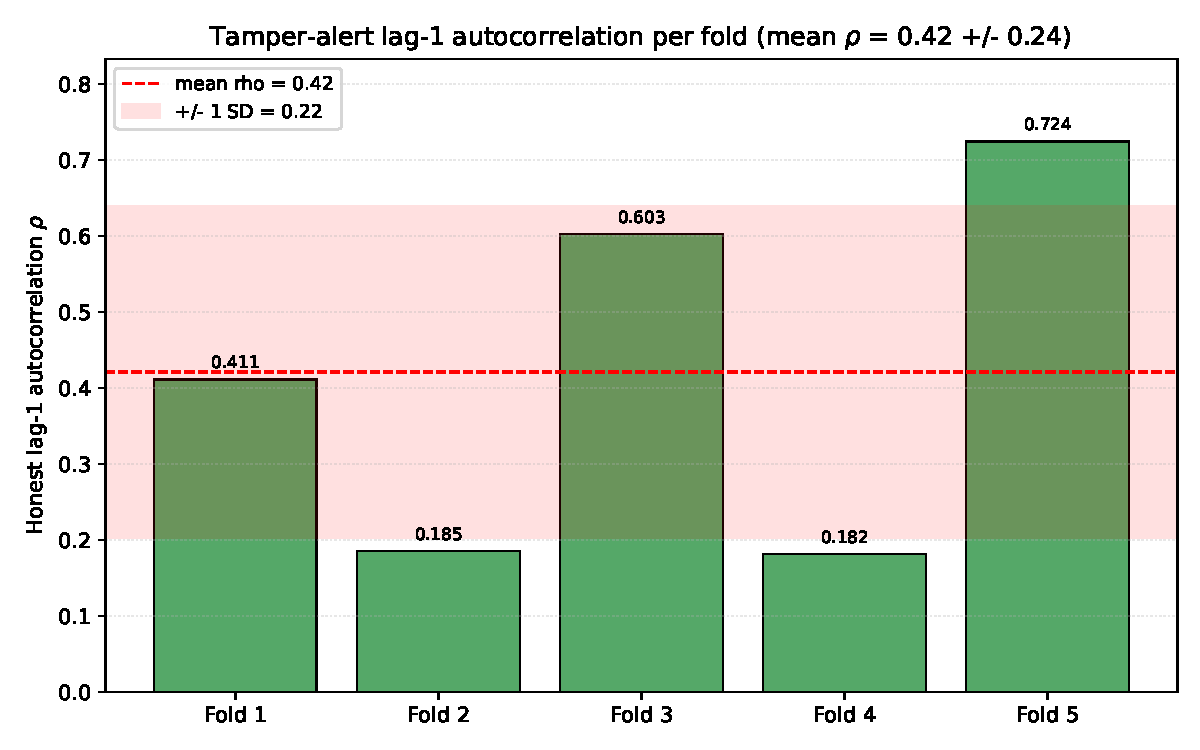
\includegraphics[width=\linewidth]{tamper_alert_autocorrelation.pdf}
  \caption{Per-fold lag-1 autocorrelation of the honest command-swap alert (bars $0.41$/$0.19$/$0.60$/$0.18$/$0.72$; mean $0.42$), the empirical value used in the deployment-relevant $K$-window aggregation.}
  \label{fig:autocorr}
\end{subfigure}
\caption{Aggregation idealization versus measurement: the row-independent curves (left) and the measured alert autocorrelation that replaces them (right).}
\label{fig:agg-pair}
\end{figure}

\paragraph{Measured autocorrelation, a sensor-vs-prior control, and the open-vocabulary operating point.} Three results materially qualify any windowed-monitoring claim and we state them as the security-relevant numbers. \emph{(1)~Measured autocorrelation.} Rather than assume $\rho$, we measured the within-source-file lag-1 autocorrelation of the honest command-swap alert on the real 5-fold AR+FSM predictions (\texttt{audit/tamper\_alert\_autocorrelation.json}): $\rho_{\text{honest}} = 0.42 \pm 0.22$ (population s.d.\ over the five folds; Figure~\ref{fig:autocorr}). Re-running the correlated aggregation at the measured honest-side $\rho$ (\texttt{audit/tamper\_aggregation\_correlated.json}, key \texttt{rho\_empirical}; the tamper-side alert autocorrelation is not separately measurable and is assumed at $\rho + 0.3 = 0.72$) gives, for command-swap at $K=10$ majority, with-metadata FPR $0.098$ at TPR $0.97$ and baseline FPR $0.184$ at TPR $0.94$; the FPR side rests on the measured value, the TPR side partly on the assumption. The deployable-operating-point claim therefore holds only in the weak sense of $\sim\!0.10$ FPR with metadata at the measured autocorrelation, not the $0.04$ best case; the honest headline figure is FPR $\approx 0.10$--$0.18$ at TPR $\approx 0.94$--$0.97$. \emph{(2)~The alert is largely prior-driven.} Substituting the corpus-modal predicted string (a sensor-\emph{independent} prediction) for the decoder output and re-scoring the command-swap detector yields TPR $0.84 \pm 0.02$ at FPR $0.39 \pm 0.02$, versus the real decoder's TPR $0.92 \pm 0.04$ at FPR $0.30 \pm 0.07$. The sensor-conditioned decoder adds only $\sim\!8$~pp of TPR and $\sim\!9$~pp of FPR-reduction over a predictor that ignores the sensors entirely: most of the row-level command-swap detectability is a property of the closed-vocabulary command \emph{prior}, not of per-instruction sensor recovery. The companion study's per-operation-class modal nulls ($0.572$ train-derived, $0.576$ test-derived, all-command-position basis~\cite{decoder_paper}) are matched to its recoverability claim, not to this detector.\footnote{The released detector flags \emph{first-command} disagreement, so the matched sensor-free null for the tamper lift is the first-command-position class-conditional modal, $\sim\!0.811$ (\texttt{audit/class\_conditional\_modal.json}); the modal-substitution control above (TPR $0.84$) operationalizes nearly this null, and the $\sim\!8$~pp lift is measured against it.} \emph{(3)~Open-vocabulary collapse.} Re-running the full tamper-injection on the nine leave-one-class-out checkpoints under deployment-true AR (\texttt{audit/threat\_model\_tamper\_loco.json}) gives command-swap FPR $0.52$ at TPR $0.85$, sign-flip FPR $0.75$ at TPR $0.14$, and feed-edit TPR $0.00$. Against an adversary not confined to trained toolpaths the command-swap detector raises a false alarm on more than half of honest windows and the sign/feed detectors are worse than useless. The security-relevant operating point is therefore the open-vocabulary one (command-swap FPR $0.52$/TPR $0.85$), with the in-distribution $K$-aggregated figures as an optimistic in-envelope ceiling.

The feed-rate detector's low FPR ($0.005$--$0.015$) is an \emph{in-distribution} artifact and does not translate to a usable detector (TPR $0.00$ under the open-vocabulary LOCO regime; Table~\ref{tab:tamper_auc}). The feed rate is also the canonical adaptive-adversary bypass field, and recovering it is not a current capability of the 4-Hz stack.

% =====================================================================
\section{The Adaptive Adversary and Structural Limits}
\label{sec:adaptive}

\paragraph{A structural bypass, not a caveat.} The monitor's blind spots are not incidental; they define a complete bypass for any adversary who knows the scheme. The recoverable fields are command identity, axis presence, and motion sign; the \emph{un}-recoverable fields are numeric coordinate value and feed rate~\cite{decoder_paper} (sign-flip and feed-edit detectors are operationally near-chance under the open-vocabulary regime, BA $\le\!0.5$ under LOCO). An adversary who keeps the command/axis/sign envelope fixed and corrupts coordinates or feed rate \emph{within the plausible in-distribution value envelope} is invisible to the per-field detector, and no $K$-window aggregation helps because the per-window signal on those fields is at chance; gross deviations retain partial in-distribution detectability (feed-edit TPR $0.22$--$0.53$, Table~\ref{tab:tamper_auc}), none under LOCO. This is exactly the high-value attack class that motivates instruction-stream verification (wrong depth of cut, wrong feed, a scrapped part or damaged tooling), so the residual security value against a non-naive adversary is small: the monitor meaningfully constrains only command/axis/sign substitutions that also stay within the trained toolpath envelope. This is a structural limitation, not a tunable parameter.

\paragraph{Sensor-side, upstream, out-of-distribution, and metadata adversaries.} Four adversary classes fall outside the monitor's scope. (i)~A \emph{sensor-side} adversary (wire-tap, EMI injection, telemetry packet-replay, calibration spoofing) can defeat the monitor by attacking the sensor path before the decoder. The operational mitigations are secured shielded wiring, EMI shielding with cross-modality consistency checks, authenticated telemetry (per-packet nonces or HMAC; IEC~62443-3-3 SR~3.1~\cite{iec62443-3-3}), and periodic offline calibration audit with multi-board cross-checks (IEC~62443-4-2 CR~3.4~\cite{iec62443-4-2}; NIST SP~800-82~Rev.~3~\cite{nist2023sp80082}). None of these attacks is benchmarked here, and a deployment that does not enforce these mitigations should not invoke the physics-of-record framing. (ii)~An \emph{upstream CAM/post-processor} adversary whose substituted toolpath stays in-vocabulary is invisible to the monitor, which agrees with the already-malicious controller stream; the system is an execution-integrity monitor, not an upstream-design-integrity monitor. (iii)~\emph{Out-of-distribution} attacks (novel command tokens, novel operation classes) have no calibrated false-alarm rate and collapse to the LOCO operating point (command-swap FPR $0.52$). (iv)~A \emph{metadata-manipulation} adversary follows from the triage point's inputs: the with-metadata configuration consumes controller-derived window-index/source-file metadata (Section~\ref{sec:operating-points}) that a controller-resident adversary can manipulate; the sensors-only baseline ($K\!=\!10$ FPR $0.184$) is the configuration robust to this adversary.

\paragraph{Limits of the verification.} The monitor cannot detect attacks whose physical effect is indistinguishable from a benign program at the 4-Hz sample rate; sub-second motion details (rapid clearance moves, small finishing passes) may be temporally aliased, with $77.7\%$ of row instances occupying at most one sample period~\cite{decoder_paper}. Mitigations (higher sample rate, additional sensor modalities, encoder retraining with row-level supervision) are open directions in the companion study's roadmap; none of them closes the adaptive-adversary bypass above, which structurally requires recovering the numeric/feed fields the present sensor stack does not carry. A separate float-epsilon target-encoding artifact in the numeric-digit pipeline (characterized in the companion limit paper~\cite{paperB_entropy} and closed by a patch) could in principle let an adversary aware of the historical encoding craft ``corrected'' G-code to trigger false alarms on a monitor trained on buggy targets; the patch closes this narrow detection-mismatch path for future deployments.

% =====================================================================
\section{Deployment Posture}
\label{sec:deployment}

\paragraph{Operating-point recommendation.} The supported posture is \textbf{forensic-support post-hoc audit, not real-time SOC monitoring}, at two operating points, never a standalone row-level real-time deployment. \textbf{(1)~Post-hoc forensic / audit:} operate the command-swap detector (sensors-only where the metadata path is untrusted) at its single measured operating point (TPR $0.92$ at FPR $0.30$ baseline; $0.95$/$0.22$ with metadata), acceptable only because the consumer is an offline analyst reviewing a contested run against the controller log, not an alert queue. The released detector is a binary per-window flag; a graded low-false-alarm operating point would require a confidence-scored detector, which the released artifacts do not provide. \textbf{(2)~Human-in-the-loop confirmation at $K\!=\!10$ majority:} adopt the measured-$\rho$ $K\!=\!10$ majority point (Section~\ref{sec:alert-budget}) only as a triage aid to a human reviewer, not as an autonomous alert. Both points hold only within the in-distribution closed-vocabulary envelope. Under the open-vocabulary LOCO regime the system is not a usable detector, and the recommendation reduces to forensic post-hoc inspection of categorical disagreements alone.

\paragraph{Usage patterns.} The monitor suits three deployment patterns. \emph{(1)~Forensic-support post-hoc audit (primary).} On suspect or contested runs, the decoded per-row G-code provides a controller-independent, physics-grounded record of executed instructions that complements the controller log; command-level disagreements (e.g.\ G0 commanded, G1 predicted; or X commanded, Y predicted) flag specific rows for offline analyst review. The reviewer is an offline analyst with the controller log in hand, not an alerting SOC tier-1 console, so the false-alarm budget that rules out real-time deployment does not apply in the same way: a $\sim$$22$~pp class-prior-controlled command increment over the history-free modal predictor ($\approx\!+13$~pp against a history-matched Markov null~\cite{decoder_paper}) is informative when it can be reviewed against a contested run rather than streamed as an alert. Numeric-value precision is too low for forensic reconstruction of coordinates; command and axis-letter disagreements are the load-bearing forensic signal. \emph{(2)~Offline process verification (secondary).} The same per-row predictions, batched over a completed run, support offline reconciliation against the commanded program as an end-of-shift / end-of-job audit step; the measured-$\rho$ $K\!=\!10$ majority point (with-metadata FPR $\sim 0.10$, TPR $\sim 0.97$) is usable as a human-in-the-loop triage aid that surfaces window blocks for a reviewer's attention, never as an autonomous alert, and never under the open-vocabulary LOCO regime. \emph{(3)~Anomaly localization within the audit pipeline (tertiary).} Operations where command-level predictions deviate from the controller's commanded program identify specific G-code lines worth investigating, complementing session-level anomaly classifiers~\cite{coelho2024anomaly,kimmell2025cnc}; the monitor is explicitly \emph{not} an autonomous real-time alerting tool.

\paragraph{Audit leverage by toolpath entropy.} The per-attack-class detectability carries a defense-in-depth corollary along an operation-class entropy axis, developed in full in the companion limit paper~\cite{paperB_entropy}: sensor-side audit is most effective on low-entropy operation classes (e.g., overruns in facing operations), is information-theoretically blind on high-entropy adaptive optimizer-generated toolpaths, and complements rather than replaces cryptographic file-hash signing. The defense-in-depth division of labor is therefore: file signing covers the program at rest, attestation covers the controller boot chain, and the sensor-side monitor covers runtime command/axis/sign substitution within the trained envelope, with each layer blind to the others' coverage.

% =====================================================================
\section{Limitations}
\label{sec:limitations}

Five limitations bound every result. First, no physical tamper was executed; the operating points derive from synthetic relabelling of honest predictions, and the false-alarm rate is the recoverability-complement proxy rather than an independent honest-run-pair measurement (Section~\ref{sec:operating-points}). Second, the detection signal is prior-dominated, with a sensor-conditioned lift of $\sim\!8$~pp TPR over a sensor-independent modal control (Section~\ref{sec:alert-budget}); claims about sensor-side security value must be read at that magnitude, not at the pooled headline accuracy. Third, all results inherit the companion study's scope: one desktop CNC platform, one material, a 4~Hz envelope-extracted stream, and a closed-vocabulary in-distribution training regime~\cite{decoder_paper}; cross-platform replication is a precondition for any deployment claim. Fourth, the open-vocabulary LOCO regime is the security-relevant boundary, and there the command-swap detector false-alarms on more than half of honest windows; the in-distribution figures are an in-envelope ceiling. Fifth, the adaptive-adversary bypass is structural: fine-grained numeric-coordinate and feed-rate tampering within the plausible value envelope is invisible to the present stack, and closing it requires sensor hardware that recovers those fields, not detector tuning (Section~\ref{sec:adaptive}). Physically-executed attack campaigns and sensor-spoofing evaluations, the regimes excluded here, are the subject of planned follow-on work.

% =====================================================================
\section{Conclusion}
\label{sec:conclusion}

We analyzed the security implications of measured per-field G-code recoverability for an out-of-band, sensor-side execution-integrity monitor. The threat model places the monitor in the Detect function as a complement to file signing and attestation, covering the residual class of runtime command/axis/sign substitution. Within that class, synthetic tamper-injection operating points show command-swap detection at balanced accuracy $0.81$--$0.86$ in-distribution, degrading to a $0.52$ false-positive rate on unseen operation classes, with sign-flip and feed-rate detection prior-driven in-distribution and at or below chance under the open-vocabulary regime. The deployment-relevant figures are the measured-autocorrelation $K\!=\!10$ triage point (FPR $0.098$ at TPR $0.97$, with metadata; the TPR side partly assumption-based, Section~\ref{sec:alert-budget}), the $\sim\!8$~pp sensor-conditioned lift over a sensor-independent modal control, and the open-vocabulary collapse; together they support forensic-support post-hoc audit and human-in-the-loop triage, and rule out real-time autonomous alerting. The monitor's blind spots define a structural bypass: an adversary who corrupts only numeric coordinates or feed rate is invisible by construction, so the highest-value attack class remains undetected on the present sensor stack. These are the quantities a next-generation stack must change, principally by recovering the numeric and feed-rate fields at a higher sample rate, before sensor-side execution verification can claim more than the audit posture supported here.

% =====================================================================
\authorcontributions{Conceptualization, S.S.E.\ and R.S.P.; methodology, S.S.E.; software, S.S.E.; validation, S.S.E.; formal analysis, S.S.E.; investigation, S.S.E.; resources, M.S.S.; data curation, S.S.E.\ and R.S.P.; writing---original draft, S.S.E.; writing---review and editing, R.S.P.\ and M.S.S.; visualization, S.S.E.; supervision, R.S.P.\ and M.S.S.; project administration, R.S.P. All authors have read and agreed to the published version of the manuscript.}

\funding{This research received no external funding.}

\institutionalreview{Not applicable.}

\informedconsent{Not applicable.}

\dataavailability{The audit artifacts cited throughout (\texttt{audit/threat\_model\_tamper\_AR\_5fold\_FSM.json}, \texttt{audit/threat\_model\_tamper\_loco.json}, \texttt{audit/tamper\_aggregation\_sweep.json}, \texttt{audit/tamper\_aggregation\_correlated.json}, \texttt{audit/tamper\_alert\_autocorrelation.json}, \texttt{audit/threat\_model\_tamper\_AR\_5fold\_FSM\_shortcuts.json}, \texttt{audit/calibration\_cross\_fold.json}, \texttt{audit/class\_conditional\_modal.json}, \texttt{audit/class\_conditional\_modal\_5fold.json}, \texttt{audit/markov\_command\_null.json}), together with the underlying sensor datasets, code, and per-fold predictions of the companion study, are publicly available at \url{https://github.com/stephenseacuello/gcode_fingerprinting} (tagged release \texttt{v1.0-submission}). Code is released under the MIT License and the 120-file aligned corpus under CC~BY~4.0.}

\acknowledgments{The authors thank the Department of Industrial and Systems Engineering at the University of Rhode Island for providing laboratory facilities and computational resources.}

\conflictsofinterest{The authors declare no conflicts of interest.}

% =====================================================================
\abbreviations{Abbreviations}{
The following abbreviations are used in this manuscript:\\

\noindent\footnotesize
AR, Autoregressive; BA, Balanced Accuracy; CAM, Computer-Aided Manufacturing; CI, Confidence Interval; CNC, Computer Numerical Control; ECE, Expected Calibration Error; EMI, Electromagnetic Interference; FPR, False Positive Rate; FSM, Finite-State Machine; HMAC, Hash-based Message Authentication Code; ICS, Industrial Control System; IEC, International Electrotechnical Commission; LOCO, Leave-One-Class-Out; NIST, National Institute of Standards and Technology; ROC, Receiver Operating Characteristic; SOC, Security Operations Center; TCB, Trusted Computing Base; TF, Teacher-Forced; TPR, True Positive Rate.
\normalsize
}

% =====================================================================
\bibliography{decoder_references.bib}

\end{document}
